\documentclass{report}
\usepackage{graphicx, tikz-cd, float, titlepic, booktabs} % Required for inserting images
\usepackage{pgfplots}
\pgfplotsset{compat=1.15}
\usepackage{mathrsfs}
\usetikzlibrary{arrows}
\usepackage{amsmath, amssymb, amsthm, amsfonts, siunitx, physics, gensymb}
\AtBeginDocument{\RenewCommandCopy\qty\SI}
\usepackage[version=4]{mhchem}
\usepackage[most,many,breakable]{tcolorbox}
\usepackage{xcolor, fancyhdr, varwidth}
\usepackage[Glenn]{fncychap}
%Options: Sonny, Lenny, Glenn, Conny, Rejne, Bjarne, Bjornstrup
\usepackage{hyperref, cleveref}
\usepackage{icomma, enumitem} %comma as decimal and continue enumerate with [resume]
\usepackage{plimsoll} %use standard state symbol with \stst
\usepackage[danish]{babel}
%%%%%%%%%%%%%%%%%%%%%%%%%%%%%%
% SELF MADE COLORS
%%%%%%%%%%%%%%%%%%%%%%%%%%%%%%
\definecolor{myg}{RGB}{56, 140, 70}
\definecolor{myb}{RGB}{45, 111, 177}
\definecolor{myr}{RGB}{199, 68, 64}
\definecolor{mytheorembg}{HTML}{F2F2F9}
\definecolor{mytheoremfr}{HTML}{00007B}
\definecolor{mylenmabg}{HTML}{FFFAF8}
\definecolor{mylenmafr}{HTML}{983b0f}
\definecolor{mypropbg}{HTML}{f2fbfc}
\definecolor{mypropfr}{HTML}{191971}
\definecolor{myexamplebg}{HTML}{F2FBF8}
\definecolor{myexamplefr}{HTML}{88D6D1}
\definecolor{myexampleti}{HTML}{2A7F7F}
\definecolor{mydefinitbg}{HTML}{E5E5FF}
\definecolor{mydefinitfr}{HTML}{3F3FA3}
\definecolor{notesgreen}{RGB}{0,162,0}
\definecolor{myp}{RGB}{197, 92, 212}
\definecolor{mygr}{HTML}{2C3338}
\definecolor{myred}{RGB}{127,0,0}
\definecolor{myyellow}{RGB}{169,121,69}
\definecolor{myexercisebg}{HTML}{F2FBF8}
\definecolor{myexercisefg}{HTML}{88D6D1}
%%%%%%%%%%%%%%%%%%%%%%%%%%%%%%%%%%%%%%%%%%%%%%%%%%%%%%%%%%%%%%%%%%%%%%
% Box environments for theorems and problems
%%%%%%%%%%%%%%%%%%%%%%%%%%%%%%%%%%%%%%%%%%%%%%%%%%%%%%%%%%%%%%%%%%%%%
\setlength{\parindent}{1cm}
%================================
% Question BOX
%================================
\makeatletter
\newtcbtheorem{question}{Opgave}{enhanced,
	breakable,
	colback=white,
	colframe=myb!80!black,
	attach boxed title to top left={yshift*=-\tcboxedtitleheight},
	fonttitle=\bfseries,
	title={#2},
	boxed title size=title,
	boxed title style={%
			sharp corners,
			rounded corners=northwest,
			colback=tcbcolframe,
			boxrule=0pt,
		},
	underlay boxed title={%
			\path[fill=tcbcolframe] (title.south west)--(title.south east)
			to[out=0, in=180] ([xshift=5mm]title.east)--
			(title.center-|frame.east)
			[rounded corners=\kvtcb@arc] |-
			(frame.north) -| cycle;
		},
	#1
}{def}
\makeatother
%================================
% DEFINITION BOX
%================================

\newtcbtheorem[]{Definition}{Definition}{enhanced,
	before skip=2mm,after skip=2mm, colback=red!5,colframe=red!80!black,boxrule=0.5mm,
	attach boxed title to top left={xshift=1cm,yshift*=1mm-\tcboxedtitleheight}, varwidth boxed title*=-3cm,
	boxed title style={frame code={
					\path[fill=tcbcolback]
					([yshift=-1mm,xshift=-1mm]frame.north west)
					arc[start angle=0,end angle=180,radius=1mm]
					([yshift=-1mm,xshift=1mm]frame.north east)
					arc[start angle=180,end angle=0,radius=1mm];
					\path[left color=tcbcolback!60!black,right color=tcbcolback!60!black,
						middle color=tcbcolback!80!black]
					([xshift=-2mm]frame.north west) -- ([xshift=2mm]frame.north east)
					[rounded corners=1mm]-- ([xshift=1mm,yshift=-1mm]frame.north east)
					-- (frame.south east) -- (frame.south west)
					-- ([xshift=-1mm,yshift=-1mm]frame.north west)
					[sharp corners]-- cycle;
				},interior engine=empty,
		},
	fonttitle=\bfseries,
	title={#2},#1}{def}
\newtcbtheorem[]{definition}{Definition}{enhanced,
	before skip=2mm,after skip=2mm, colback=red!5,colframe=red!80!black,boxrule=0.5mm,
	attach boxed title to top left={xshift=1cm,yshift*=1mm-\tcboxedtitleheight}, varwidth boxed title*=-3cm,
	boxed title style={frame code={
					\path[fill=tcbcolback]
					([yshift=-1mm,xshift=-1mm]frame.north west)
					arc[start angle=0,end angle=180,radius=1mm]
					([yshift=-1mm,xshift=1mm]frame.north east)
					arc[start angle=180,end angle=0,radius=1mm];
					\path[left color=tcbcolback!60!black,right color=tcbcolback!60!black,
						middle color=tcbcolback!80!black]
					([xshift=-2mm]frame.north west) -- ([xshift=2mm]frame.north east)
					[rounded corners=1mm]-- ([xshift=1mm,yshift=-1mm]frame.north east)
					-- (frame.south east) -- (frame.south west)
					-- ([xshift=-1mm,yshift=-1mm]frame.north west)
					[sharp corners]-- cycle;
				},interior engine=empty,
		},
	fonttitle=\bfseries,
	title={#2},#1}{def}

\newtcbtheorem{theo}%
    {Theorem}{}{theorem}
\newtcolorbox{prob}[1]{colback=red!5!white,colframe=red!50!black,fonttitle=\bfseries,title={#1}}
%================================
% NOTE BOX
%================================

\usetikzlibrary{arrows,calc,shadows.blur}
\tcbuselibrary{skins}
\newtcolorbox{note}[1][]{%
	enhanced jigsaw,
	colback=gray!20!white,%
	colframe=gray!80!black,
	size=small,
	boxrule=1pt,
	title=\textbf{Note:},
	halign title=flush center,
	coltitle=black,
	breakable,
	drop shadow=black!50!white,
	attach boxed title to top left={xshift=1cm,yshift=-\tcboxedtitleheight/2,yshifttext=-\tcboxedtitleheight/2},
	minipage boxed title=1.5cm,
	boxed title style={%
			colback=white,
			size=fbox,
			boxrule=1pt,
			boxsep=2pt,
			underlay={%
					\coordinate (dotA) at ($(interior.west) + (-0.5pt,0)$);
					\coordinate (dotB) at ($(interior.east) + (0.5pt,0)$);
					\begin{scope}
						\clip (interior.north west) rectangle ([xshift=3ex]interior.east);
						\filldraw [white, blur shadow={shadow opacity=60, shadow yshift=-.75ex}, rounded corners=2pt] (interior.north west) rectangle (interior.south east);
					\end{scope}
					\begin{scope}[gray!80!black]
						\fill (dotA) circle (2pt);
						\fill (dotB) circle (2pt);
					\end{scope}
				},
		},
	#1,
}
%================================
% EXAMPLE BOX
%================================
\newtcbtheorem[number within=section]{Example}{Example}
{%
	colback = myexamplebg
	,breakable
	,colframe = myexamplefr
	,coltitle = myexampleti
	,boxrule = 1pt
	,sharp corners
	,detach title
	,before upper=\tcbtitle\par\smallskip
	,fonttitle = \bfseries
	,description font = \mdseries
	,separator sign none
	,description delimiters parenthesis
}
{ex}
%================================
% THEOREM BOX
%================================

\tcbuselibrary{theorems,skins,hooks}
\newtcbtheorem[number within=section]{Theorem}{Theorem}
{%
	enhanced,
	breakable,
	colback = mytheorembg,
	frame hidden,
	boxrule = 0sp,
	borderline west = {2pt}{0pt}{mytheoremfr},
	sharp corners,
	detach title,
	before upper = \tcbtitle\par\smallskip,
	coltitle = mytheoremfr,
	fonttitle = \bfseries\sffamily,
	description font = \mdseries,
	separator sign none,
	segmentation style={solid, mytheoremfr},
}
{th}

%%%%%%%%%%%%%%%%%%%%%%%%%%%%%%%%%%%%%%%%%%%%%%%%%%%%%%%%%%%%%%%%%
% SELF MADE COMMANDS
%%%%%%%%%%%%%%%%%%%%%%%%%%%%%%
\newcommand{\sol}{\setlength{\parindent}{0cm}\textbf{\textit{Løsning:}}\setlength{\parindent}{1cm}}
%%%%%%%%%%%%%%%%%%%%%%%%%%%%%%%%%
\usepackage[tmargin=2cm,rmargin=1in,lmargin=1in,margin=0.85in,bmargin=2cm,footskip=.2in]{geometry}\pagestyle{fancy}
\lhead{Minrui Kevin Zhou 3.b}
\rhead{Opgavesæt 1}

\title{Opgavesæt 1\\
{\Large \textbf{3.b kemi A}}}
\author{Kevin Zhou}
\date{\today}

\begin{document}
\maketitle
\begin{note}
  Databog fysik kemi (2007) er benyttet ved beregningerne.
\end{note}
\section*{Opgave 1: Aromastoffer i oregano}
\sol \\
\textbf{a.}
2-(4-methylphenyl)propan-1-ol, som ses i \cref{fig:isomer} er en strukturisomer til carvacrol, da de har samme molekylformel, men forskellig strukturformler.
Isomeren er også en primær alkohol, da hydroxy-gruppen sidder på et endestillet \ce{C}-atom i en alifatisk \ce{C}-kæde.
\begin{figure}[H]
\begin{center}
  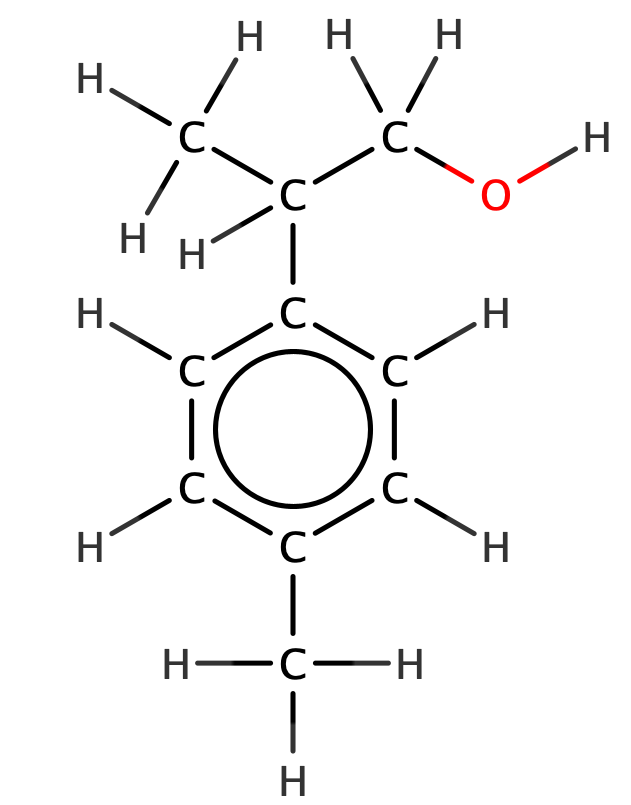
\includegraphics[scale=0.3]{isomer.png}
\end{center}
  \caption{2-(4-methylphenyl)propan-1-ol tegnet i MarvinSketch}
\label{fig:isomer}
\end{figure}
\textbf{b.}
De funktionelle grupper markeret i de fire stoffer ses i \cref{fig:funktionel}.
\begin{figure}[H]
\begin{center}
  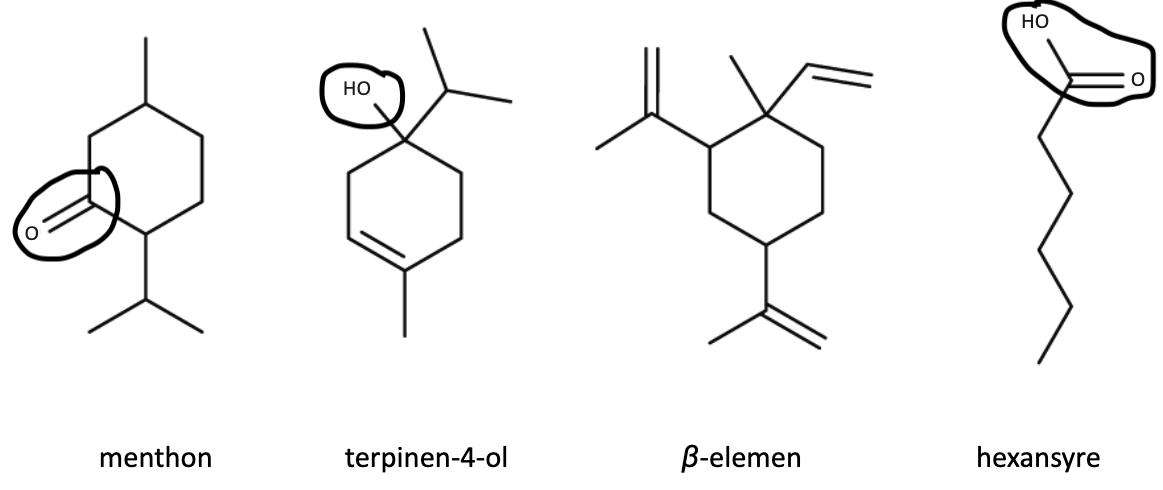
\includegraphics[scale=0.3]{funktionelle_grupper.png}
\end{center}
\caption{De funktionelle grupper markeret med en bolle omkring sig}
\label{fig:funktionel}
\end{figure}
Det er da klart, at menthon er en keton, terpinen-4-ol er en alkohol, hexansyre er en carboxylsyre og $\beta$-elemen (som er et carbonhydrid) ikke indeholder nogen funktionelle grupper.

\section*{Opgave 1: Nitrat i grundvand}
\sol \\
\textbf{a.}
Den formelle stofmængdekoncentration af kaliumnitrat må være
\begin{equation*}
\begin{split}
  c \left(\ce{KNO3} \right) &=\frac{m(\ce{KNO3} ) }{V\cdot M(\ce{KNO3} )}\\
  &=\frac{0,506 \;\unit{g} }{0,250 \;\unit{L} \cdot 101,10 \;\unit{g/mol} }\\
  &\approx 0,0200 \;\unit{\textsc{m}} 
\end{split}
\end{equation*}
Altså har vi $c(\ce{KNO3})=0,0200 \;\unit{\textsc{m}} $.\\[1ex]
\textbf{b.}
2-hydroxybenzoesyre (salicylsyre) har $pK_s=2,98$ ved $25 \;\unit{\celsius} $.
Der gælder da
\begin{equation*}
\begin{split}
  K_s=\frac{\left[\ce{H3O+} \right]^2}{c_s-\left[\ce{H3O+} \right]} &\implies \left[\ce{H3O+} \right]=\frac{-K_s + \sqrt{K_s^2 - 4 \cdot \left(-K_s \cdot c_s\right) } }{2}\\
  &\iff pH=- \log\left(\frac{-K_s + \sqrt{K_s^2 - 4 \cdot \left(-K_s \cdot c_s\right) } }{2 \;\unit{\textsc{m}} }\right) 
\end{split}
\end{equation*}
Vi kan nu regne pH ud med $K_s=10^{-pK_s} \;\unit{\textsc{m}} =10^{-2,98} \;\unit{\textsc{m}} $.
\begin{equation*}
\begin{split}
  pH&=- \log\left(\frac{-K_s + \sqrt{K_s^2 - 4 \cdot \left(-K_s \cdot c_s\right) } }{2 \;\unit{\textsc{m}} }\right) \\
  &=- \log\left(\frac{-10 ^{-2,98} \;\unit{\textsc{m}} +\sqrt{\left(10 ^{-2,98} \;\unit{\textsc{m}} \right)^2 - 4 \cdot \left(-10 ^{-2,98} \;\unit{\textsc{m}} \cdot 0,018 \;\unit{\textsc{m}} \right) } }{2 \;\unit{\textsc{m}} }\right) \\
  &\approx 2,4
\end{split}
\end{equation*}
Altså er pH i den mættede salicylsyreopløsning $2,4$.\\[1ex]
\textbf{c.}
Det ses fra resultaterne, at absorbansen generelt er maksimal ved bølgelængden $411 \;\unit{nm} $.
Absorbanserne målt ved de forskellige koncentrationer sættes ind i Logger Pro, hvor vi laver en ligefrem proportionel regression (grundet Lambert Beers lov), hvilket kan ses i \cref{fig:absorbans}.
\begin{figure}[H]
\begin{center}
  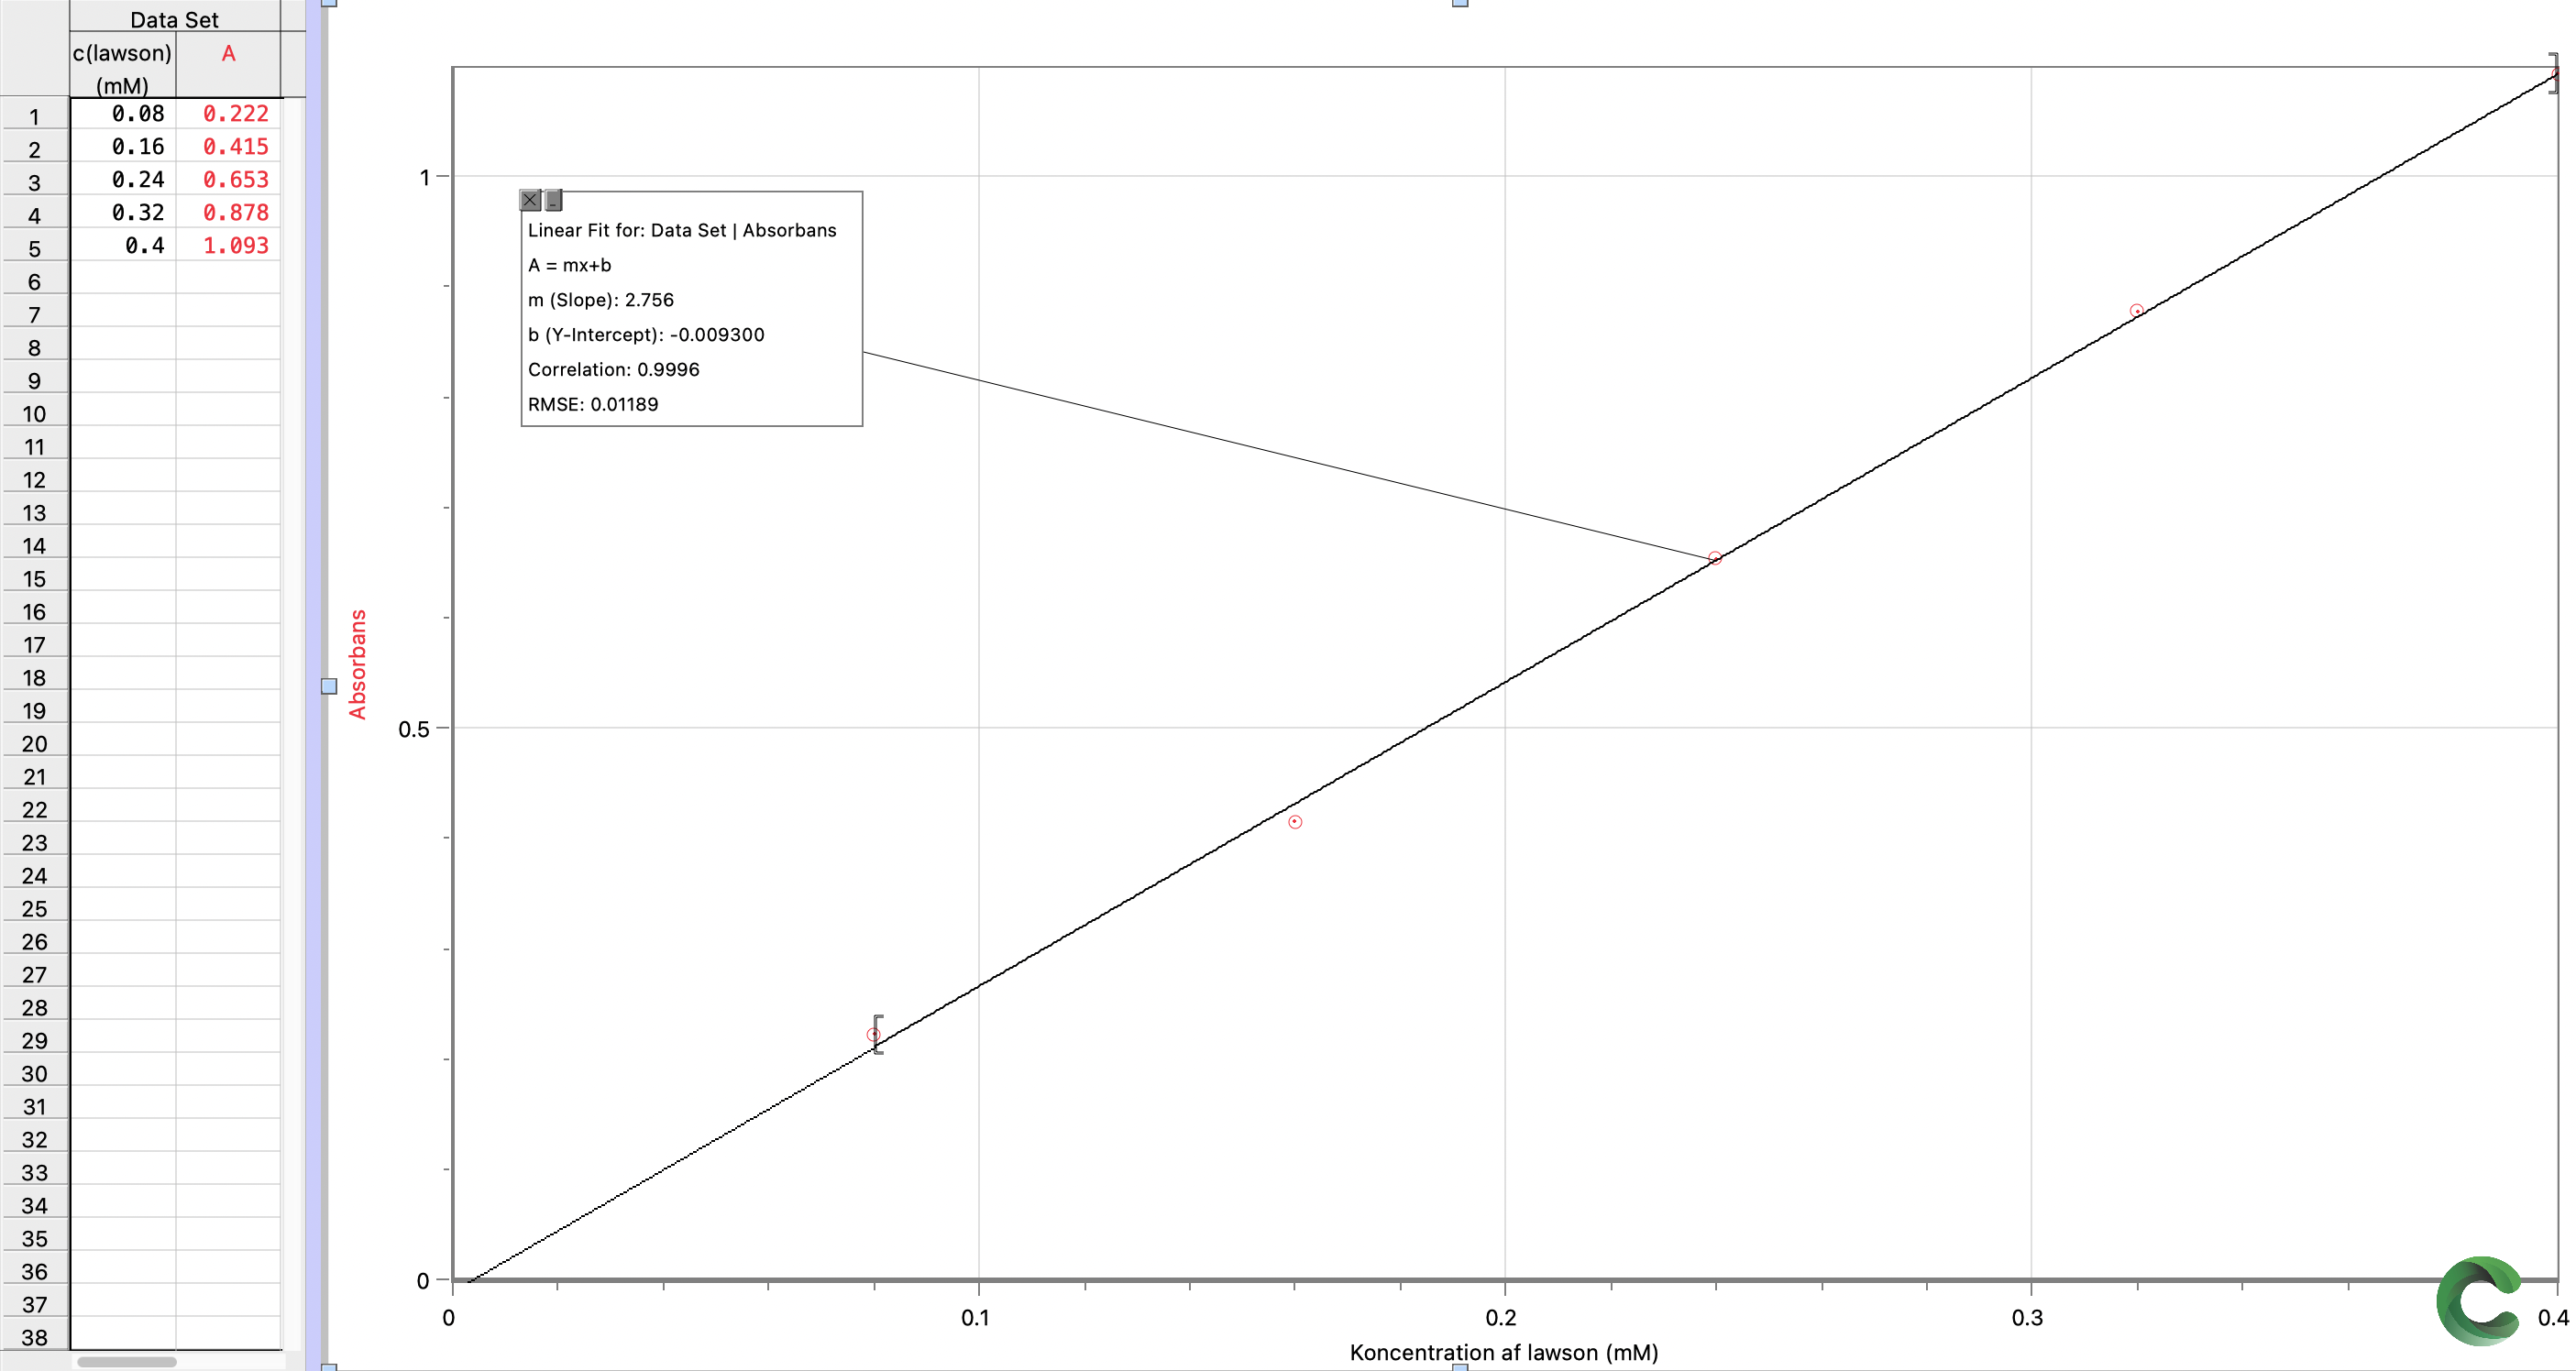
\includegraphics[scale=0.3]{absorbans.png}
\end{center}
\caption{Sammenhængen mellem absorbansen og koncentrationen af \ce{KNO3} findes med Logger Pro}
\label{fig:absorbans}
\end{figure}
Fra vores regression har vi
\[
A=0,1529 \;\unit{\frac{1}{m \textsc{m}}} \cdot c(\ce{KNO3} )\iff c(\ce{KNO3} )=\frac{A}{0,1529}\;\unit{m \textsc{m}} 
\] 
Vi kan nu regne den formelle koncentration af kaliumnitrat i vandprøven ud.
\begin{equation*}
\begin{split}
  c(\ce{KNO3} )&=\frac{A}{0,1529}\;\unit{m \textsc{m}} \\
  &=\frac{0,960}{0,1529} \;\unit{m \textsc{m}} \\
  &=6,27861 \;\unit{m \textsc{m}} 
\end{split}
\end{equation*}
Siden $\left[\ce{NO3-} \right]=c(\ce{KNO3} )$, så gælder der, at indholdet af nitrat må være
\begin{equation*}
\begin{split}
  [\ce{NO3-} ] \cdot M(\ce{NO3-} ) &= c(\ce{KNO3} ) \cdot M (\ce{NO3-} ) \\
  &=6,27861 \;\unit{m \textsc{m}} \cdot 62,00 \;\unit{g/mol} \\
  &\approx 3,9 \cdot 10^2 \;\unit{mg/L} 
\end{split}
\end{equation*}
Vi har altså bestemt indholdet af nitrat i vandprøven til at være $3,9 \cdot 10^2 \;\unit{mg/L} $.

\section*{Opgave 2: IVA - en genetisk stofskiftesygdom}
\sol \\
\textbf{a.}
3-methylbutansyre har $pK_s=4,77$ ved $25 \;\unit{\celsius} $.
Da det er en svag syre, kan vi uden at det medfører større fejl regne pH med
\begin{equation*}
\begin{split}
  pH&=\frac{1}{2} \cdot \left(pK_s- \log\left(\frac{c_s}{\unit{\textsc{m}}}\right) \right) \\
  &=\frac{1}{2} \cdot \left(4,77 - \log\left(\frac{0,15 \;\unit{\textsc{m}} }{\unit{\textsc{m}}}\right) \right) \\
  &\approx 2,8
\end{split}
\end{equation*}
Altså er pH i opløsningen $2,8$.\\[1ex]
\textbf{b.}
Vi finder først et udtryk for den formelle stofmængdekoncentration af syren.
\begin{equation*}
\begin{split}
  pH=\frac{1}{2} \cdot \left(pK_s- \log\left(\frac{c_s}{\unit{\textsc{m}}}\right) \right) &\iff \log\left(\frac{c_s}{\unit{\textsc{m}}}\right) =pK_s-2 \cdot pH\\
  &\iff c_s=10 ^{pK_s-2 \cdot pH} \;\unit{\textsc{m}} 
\end{split}
\end{equation*}
Den del af isovalerianesyre (som vi betegner $S$), der findes på syreform, når vi ser bort fra vands selvionisering, i urin må være
\begin{equation*}
\begin{split}
  x_s&=1-\alpha(S)\\
  &=1-\frac{[\ce{H3O+} ]}{c_s}\\
  &=1-\frac{10 ^{-pH} \;\unit{\textsc{m}} }{10 ^{pK_s-2 \cdot pH} \;\unit{\textsc{m}}}\\
  &=1-10^{pH-pK_s}\\
  &=1-10 ^{4,5-4,77}\\
  &\approx 0,46\\
  &=46 \%
\end{split}
\end{equation*}
Altså findes 46 \% af isovalerianesyre på syreform ved pH 4,5 og ved $25 \;\unit{\celsius} $.\\[1ex]
\textbf{c.}
Stofmængden af henholdsvis C, H, N og O må være
\begin{equation*}
\begin{split}
  &n(\ce{C})=\frac{m(\ce{C})}{M(\ce{C})}=\frac{52,82 \;\unit{g} }{12,01 \;\unit{g/mol} }=4,3980 \;\unit{mol}  \\
  &n(\ce{H})=\frac{m(\ce{H})}{M(\ce{H})}=\frac{8,23 \;\unit{g} }{1,01 \;\unit{g/mol} }=8,1485 \;\unit{mol} \\
  &n(\ce{N})=\frac{m(\ce{N})}{M(\ce{N})}=\frac{8,80 \;\unit{g} }{14,01 \;\unit{g/mol} }=0,6281 \;\unit{mol} \\
  &n(\ce{O})=\frac{m(\ce{O})}{M(\ce{O})}=\frac{30,15 \;\unit{g} }{16,00 \;\unit{g/mol} }=1,8844 \;\unit{mol} 
\end{split}
\end{equation*}
Vi beregner nu stofmængdeforholdene ved at dividere den mindste stofmængde op i de øvrige.
\begin{equation*}
\begin{split}
  &\frac{n(\ce{C} )}{n(\ce{N} )}=\frac{4,3980 \;\unit{mol} }{0,6281 \;\unit{mol} }=7,002 \approx 7\\
  &\frac{n(\ce{H} )}{n(\ce{N} )}=\frac{8,1485 \;\unit{mol} }{0,6281 \;\unit{mol} }=12,97 \approx 13\\
  &\frac{n(\ce{O} )}{n(\ce{N} )}=\frac{1,8844 \;\unit{mol} }{0,6281 \;\unit{mol} }=3,000 \approx 3
\end{split}
\end{equation*}
Stoffet B's molekylformel må altså være af formen
\[
\ce{(C7H13NO3)_x} 
\] 
Da vi kender B's molare masse, kan vi beregne $x$
\begin{equation*}
\begin{split}
  x&=\frac{M(B)}{M(\ce{C7H13NO3})}\\
  &=\frac{159,18 \;\unit{g/mol} }{159,18 \;\unit{g/mol} }\\
  &=1
\end{split}
\end{equation*}
Altså må molekylformlen for B være
\[
\ce{C7H13NO3} 
\] 
Ved en kondensationsreaktion sker en sammenbinding af to organiske molekyler under fraspaltning af et vandmolekyle.
Da giver molekylformlen for B mening, hvis stoffet dannes ved en kondensationsreaktion mellem glycin og isovalerianesyre. 
En mulig struktur for B ses da i \cref{fig:B}.
\begin{figure}[H]
\begin{center}
  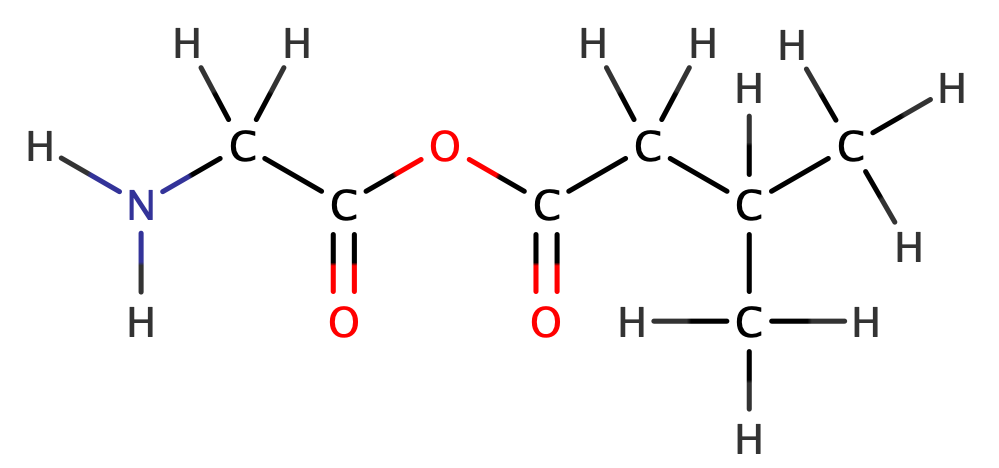
\includegraphics[scale=0.4]{B.png}
\end{center}
\caption{En mulig strukturformel for B tegnet i MarvinSketch}
\label{fig:B}
\end{figure}

\end{document}
